% !TEX root = dissertation_BB.tex
%% spellcheck-language en-US

%   #
%  ##
%   #
%   #
%  ###

\chapter{Light-sheet imaging of mammalian development}

\graphicspath{{./figures/1_spim/}}

Understanding mammalian development has been a long standing challenge for developmental biologists and medical professionals alike. Understanding early embryonic development allows to shed light on questions such as human infertility and congenital diseases \cite{todo}. 
This phase of early life is an incredibly complex and dynamic process spanning through large scales in space and time. Subcellular processes at the nanoscale are happening in the range of milliseconds or faster, while whole embryo reorganizations and tissue migration events take place over the course of hours \cite{gilbert_developmental_2013}. Resolving these processes presents a true challenge, since to also understand the underlying mechanisms molecular specificity is just as crucial as high spatial and temporal resolution.

Fluorescence microscopy \cite{diaspro_optical_2011}

The most commonly used model organism for these kind of questions is the mouse embryo, that exhibits several common features to human development, and allows to study it 
It has several advantages: full genome is sequenced \cite{mouse_genome_sequencing_consortium_initial_2002}, relatively fast reproduction rate facilitating genetic modifications, already extensively developed tools for genetics and handling \cite{capecchi_new_1989,silver_mouse_1995}. All of these make the mouse embryo the primary model organism when investigating biological processes in mammalians.

fixed samples, histology, immunofluorescence -> no time lapse

ex vivo embryo culture

Hooke's Micrographia 1665 \cite{hooke_micrographia:_1665}

Imaging mouse embryonic development is an extremely challenging task, due to the intrauterine development of embryos. Although this prevents direct access to the embryos, for some developmental stages it is possible to culture them in an \textit{ex vivo} environment using special media and carefully controlled environmental conditions \cite{garcia_live_2011,doherty_culture_2000}. A second hurdle, aside from \textit{in vitro} culturing, arises from the extreme light sensitivity \cite{nowotschin_chapter_2010} of these embryos, hindering the possibility of long term time-lapse experiments in standard confocal microscopes. Even a few hours of imaging every \SI{15}{mins} can impair or arrest normal development \cite{strnad_inverted_2016}.

Despite these difficulties, numerous studies successfully used confocal microscopy to image live embryos in an \textit{ex vivo} environment, although these studies typically only 

mostly wide-field, Oct4 - self renewal of pluripotent stem cells in ICM/epiblast \cite{nichols_formation_1998}

Sox2 in ICM, also maternal proteins important, similar role as Oct4 Both Oct4 and Sox2 are necessary for ICM formation, without cells become trophoectoderm. Furthermore, for extraembryonic endoderm (ExEn) only Oct4 is required, while for extraembryonic ectoderm (ExE) only Sox2 is required. No time lapse, but confocal used to locate proteins in embryo \cite{avilion_multipotent_2003}

inactivation of X chromosome and histone macroH2A1
mouse liver in confocal - fixed samples \cite{costanzi_histone_1998}

antibodies against amyloid $\upbeta$-peptide reduce Alzheimer in mouse, cryostat sections of mouse brain imaged in confocal\cite{bard_peripherally_2000}


aorta imaging in embryo slices, confocal, live stem cells from aorta endothelium? \cite{boisset_vivo_2010}

fixed embryos, maintaining pluripotency in embryonic stem cells\cite{sato_maintenance_2004}

imaging thrombus formation in real time with intravital high-speed confocal microscopy\cite{falati_real-time_2002}

turning blood into brain hematopoietic stem cells migrate to brain and express neuron-specific antigens \cite{mezey_turning_2000}

uj regi cikk Keller \cite{keller_life_2006}


Light microscopy is one of the oldest methods that is still widely used today to investigate the inner workings of microscopic life. Light-sheet microscopy is a relatively new addition to the arsenal of tools that comprise light microscopy methods, and is especially suitable for live imaging of embryonic samples over extended periods of time \cite{krzic_multiview_2012,tomer_quantitative_2012}. It is also easily adapted to the sample, allowing to image a large variety of specimens, from entire organs, such as cleared mouse brains \cite{dunsby_optically_2008}, to the subcellular processes occurring inside cultured cells \cite{capoulade_quantitative_2011}.

basic concept of spim
\begin{figure}[hbt]
    \centering
    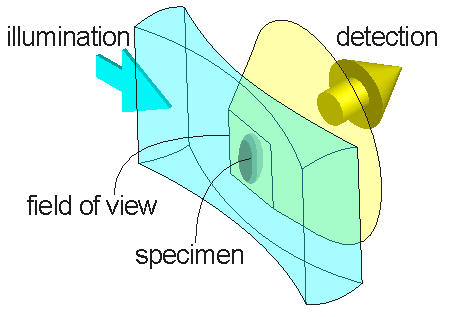
\includegraphics[width=0.6\textwidth]{spim_concept}
    \caption{\textbf{Basic concept of single-plane illumination microscopy.} The sample is illuminated from the side by laser light shaped to a light-sheet (blue). This illuminates the focal plane of the detection lens, that collects light in a wide-field mode (yellow). The image is recorded, and the sample is translated through the light-sheet to acquire an entire 3D stack.}
    \label{fig:spim_concept}
\end{figure}

\section{Fluorescence microscopy}
Fluorescence microscopy \cite{lichtman_fluorescence_2005} very small amount of illumination photons will result in fluorescence ($<0.0001\%$), the signal to noise ratio of the fluorescence is still very high due to the filtering.

good for live, naturally fluorescent structures

autofluorescence not specific
fluorescent dyes
fluorescent proteins
Nobel Prize in chemistry in 2008 GFP \cite{service_three_2008}
lot of fluorescent proteins since then \cite{shaner_guide_2005}. 
benefits: cell is producing
using genetic techniques possible to bind to other proteins, and specifically label structures of interest

\subsection{Wide-field fluorescence microscopy}
(Figure \ref{fig:wide-field})
regular microscope -> figure for this?
filter cube

\begin{figure}[htbp]
    \centering
    \includegraphics[page=4,scale=0.8]{spim_cyl}
    \caption{\textbf{Wide-field fluorescent microscope.}}
    \label{fig:wide-field}
\end{figure}

\subsubsection{Resolution of a wide-field microscope}

resolution
smallest distance of two points still distinguishable
few different definitions
this is because of diffraction
Airy pattern
Rayleigh criterion -> Abbe's formula \cite{abbe_beitrage_1873}
$d = 0.61 \frac{\lambda}{NA}$
plus axial resolution
$d_z = \frac{2\lambda}{NA^2}$

this result is base on the paraxial approximation of the Helmholtz equation, thus only apply for small NA.
a more general method to calculate resolution for high NA imaging systems is SGH:
A generally accepted method to calculate lateral ($\sigma_{xy}$) and axial ($\sigma_{z}$) resolution of an optical microscope is described by the Stelzer-Grill-Heisenberg, or SGH~theory\cite{grill_method_1999, stelzer_uncertainty_2000}:
A more general expression, works for large NA as well
\begin{equation} \label{eq:latres}
\sigma_{xy}=\frac{\lambda}{\sqrt{3-2 \cos \alpha - \cos 2 \alpha}}
\end{equation}
\begin{equation} \label{eq:axres}
\sigma_z = \frac{\lambda}{1-\cos \alpha}
\end{equation}
Generally, instead of $\alpha$, the numerical aperture (NA) is commonly used to characterize a lens' aperture. 
$NA=n\cdot \sin \alpha$, where n is the refractive index of the medium and $\alpha$ stands for the angular aperture.

even for high NA axial/lateral ratio $\sim 3-6$ (Figure~\ref{fig:resolution})
In principle it is possible to achieve isotropic resolution by increasing the acceptance angle to $\alpha = 180^\circ$, which means all light needs to be collected from the sample. Designing an objective that is capable of this feat, however, is currently beyond our technological capabilities, furthermore is would require an alternative method for sample positioning, since mechanical translation is not possible in such a configuration. One attempt at such an imaging system was the Multi-Imaging Axis Microscopy (MIAM) \cite{swoger_multiple_2003,swoger_multi-view_2007} that consisted of 4 identical objectives arranged in a tetrahedral fashion to collect as much light as possible from multiple directions. 

Another disadvantage of the wide-field microscope, is that it can not be used with thick specimens. Usually this type of microscopy is only used for a single layer of cells, because all the objects in the field of view will appear on the imaging plane, not just the plane in focus. These objects will appear blurred if close to the focus, or just evenly add to the background noise if they are further from the focus. This is why imaging specimens much thicker than $10\ \mu m$ will result in suboptimal image quality.

\begin{figure}[htpb]
    \centering
    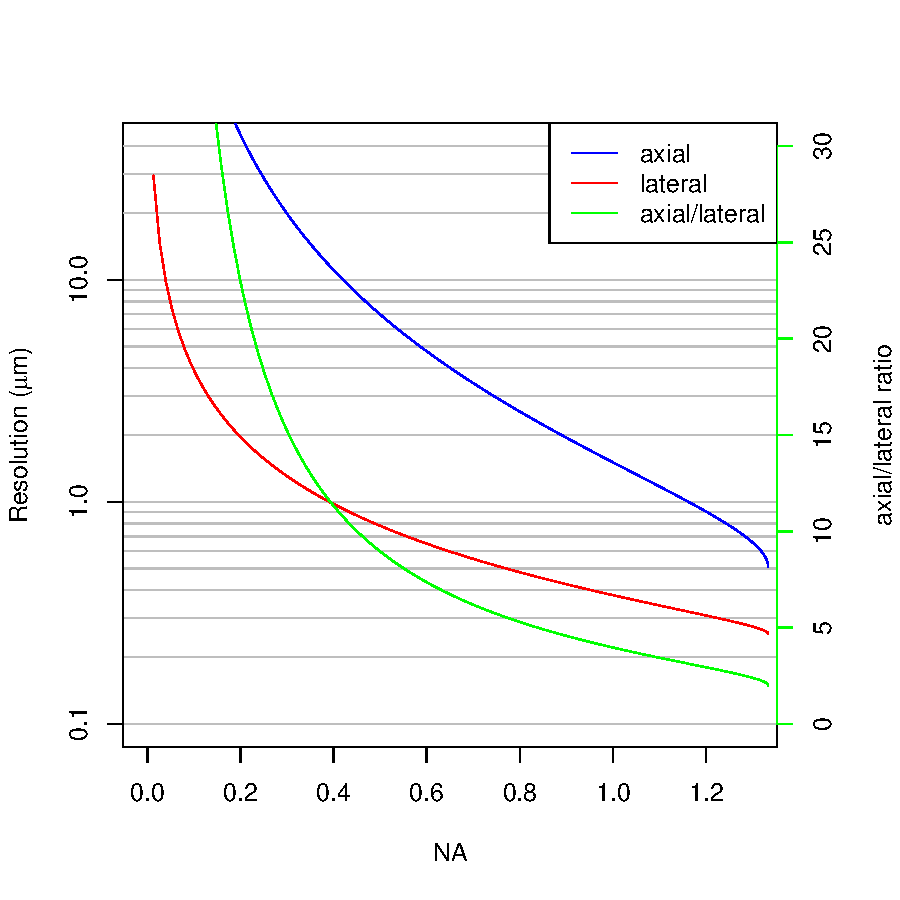
\includegraphics[width=0.6\textwidth]{resolution}
    \caption{\textbf{Resolution of a wide-field microscope.} Axial (blue) and lateral (red) resolutions of a wide-field microscope are shown with respect to the numerical aperture (NA). Resolutions are calculated with $\lambda =510nm$, the emission maximum of GFP and $n=1.333$, the refractive index of water, for water dipping objectives.}
    \label{fig:resolution}
\end{figure}

\subsection{Confocal microscopy}

Laser scanning confocal microscopy \cite{davidovits_photomicrography_1973} addresses the problem of noise originating from the out of focus planes. The principle for illumination and detection optics is very similar to a wide-filed microscope, but for illumination a focused laser light is used.

The biggest change is in the detection method: the confocal microscope uses a pinhole, to exclude light coming from out of focus planes. Since only those rays are taking part in the imaging that originate from the focus, the image quality is highly improved. This microscopy technique is also capable of 3D imaging, with an axial resolution corresponding to a wide-filed microscope.

However, the image can not be registered as simply as with the wide-filed detection, since at any given time, only a very small portion of the sample will be used in the imaging. Because of this, a more sensitive detection is required, which generally means the use of a photomultiplier. To get the whole image, the focus is scanned through the whole sample (or rather, the sample is scanned through the focus), recording an intensity value for each position. The image is then generated using a computer based on the recorded position and intensity values.


Although this microscopy technique already has 3D capabilities, it's axial resolution is still limited by the SGH theory, since it uses only one objective. Imaging live specimens for an extended period of time with confocal microscopy although possible \cite{aldaz_live_2010}, is not ideal. Since for each voxel imaged, almost the entire specimen has to be illuminated, which results in a very high dose of radiation of the samples. This can be as much as 30--100 times bigger, than the dose used for the actual imaging \cite{reynaud_light_2008}. High power of laser for an extended time frame can result in bleaching the fluorophores, thus resulting in a lower signal at later times, but the more significant issue is phototoxicity, that is when the cells themselves are damaged by the laser light.

\begin{figure}
\begin{subfigure}[t]{0.49\textwidth}
    \centering
    \includegraphics[page=3,width=\textwidth]{spim_cyl}
    \caption{\textbf{Confocal microscope}}
    \label{fig:confocal}
\end{subfigure}
\begin{subfigure}[t]{0.49\textwidth}
    \centering
    \includegraphics[page=5,width=\textwidth]{spim_cyl}
    \caption{\textbf{Confocal-theta microscope}}
    \label{fig:conf-theta}
\end{subfigure}
\caption{\textbf{Basic optical components of a laser scanning confocal and confocal-theta microscope.} Both type of microscopes use confocal images detection, which means that a pinhole is used to exclude light coming from out of focus points. Light intensity is measured by a photomultiplier for every voxel in the region of interest. The final image is generated on a computer using the positions and recorded intensity values. A regular confocal microscope (\ref{fig:confocal}) uses the same objective for illumination and detection, while a confocal-theta microscope (\ref{fig:conf-theta}) uses a second objective that is rotated by $\vartheta$ around the focus. In this case, $\vartheta = 90^\circ$.}
\label{fig:confocals}
\end{figure}

\subsection{Confocal-theta microscopy}

Although confocal microscopy already provides a better resolution in all dimensions, the ratio of the axial and lateral resolution is still very high, due to the single objective illumination and detection. This seriously limits the microscope's 3D imaging capabilities, since in the $z$ direction (i.e. along the imaging axis) the resolution would be significantly worse than in the other directions.

Confocal-theta microscopy \cite{stelzer_fundamental_1994} introduces a second objective to a regular confocal microscope, that is used to illuminate the sample (Figure \ref{fig:conf-theta}). Since this decouples the illumination and detection, using a filter cube is no longer necessary. The second objective is rotated by $\vartheta$ around the focus, this is the where the name of this setup originates.

Resolution is also improved compared to the regular confocal microscope, because the lateral resolution of the imaging objective now corresponds to the axial resolution of the detection objective. The combined resolution of the two-objective system can be calculated in the following manner \cite{krzic_multiple-view_2009}:
\begin{equation}
\frac{1}{\sigma _{sys}^2} = \frac{1}{\sigma _{ill}^2} + \frac{1}{\sigma _{det}^2}
\end{equation}
where $\sigma_{ill} = \sigma_{xy}$ and $\sigma_{det} = \sigma_z$ for the axial resolution of the system, and reversed for the lateral resolution of the system. This means, that the axial and lateral resolution would be the same (if the same objectives are used), and the resulting point spread function is almost isotropic.

Although this is a big improvement to confocal microscopy, the issue of photobleaching and phototoxicity is still not solved with a confocal theta microscope, which means that longer developmental processes are near impossible to follow with this type of microscopy.




\section{Light-sheet microscopy}
\label{sec:light-sheet}
One main drawback of the point scanning methods introduced in the previous section is the inefficiency of the illumination scheme. Although almost the whole sample is illuminated, information is only collected from the focal volume. This results in two main limiting factors: acquisition speed depends on the point scanning speed, which in turn is inversely proportional to the signal to noise ratio. Furthermore, because of the inefficiency of the illumination scheme, photobleaching and phototoxic effects further reduce the usability of these techniques for live imaging, especially for long term experiments \cite{}.



The main principle behind single plane illumination microscopy, that is illuminating the sample from the side by a very thin light-sheet, dates back to the early 20\textsuperscript{th} century, when Siedentopf and Zsigmondy first described the ultramicroscope \cite{siedentopf_uber_1902}. This microscope used sunlight as an illumination source, that was guided through a precision slit to generate a thin light-sheet. This allowed Zsigmondy to visualize gold nanoparticles floating in and out of the light-sheet. Since these particles are much smaller than the wavelength of the light, the device was called an ultramicroscope. His studies with colloids together with the development of the ultramicroscope led Zsigmondy to win the Nobel Prize in 1925.

previous to SPIM:
Voie et al. fixed guinea pig cochlea, rotating and reconstruction in 3D \cite{voie_orthogonal-plane_1993}, called Orthogonal-plane Fluorescent Optical Sectioning. Lateral resolution around \SI{10}{\micro m} and axial resolution of \SI{26}{\micro m}, with very large, \SI{1.5}{mm} field of view. Since the specimens they imaged contained calcium rich bone tissue, optical imaging was only possible by using an optical clearing method. In this work, they used EDTA (ethylenediaminetetraacetic acid) dehydrated in ethyl alcohol, then it was cleared, finally immersed in a fluorescent dye bath. TO acquire 3D images, the specimen was rotated, and translated to compensate for the off-axis rotation.

follow-up to Voie and Spelman: \cite{voie_three-dimensional_1995} 3D reconstruction of the cochlea for the images

Similar to SPIM but not fluorescent: light scanning photomicrography \cite{huber_3d_2001}

Then, in 2002, Fuchs et al. introduces Thin  Light-Sheet Microscopy \cite{fuchs_thin_2002} who use this technique to investigate the microbial life in seawater samples without disturbing their natural environment (by e.g. placing them on a coverslip). Using TSLM allowed the to image the bacteria directly in the staining solution containing SYBR Green I without having to deal with background illumination from the dye, which would have been an issue with confocal microscopy for example. Their light-sheet was similar to the one utilized in OPFOS, being \SI{23}{\micro m} thin, and providing a \SI{1}{mm} \ \SI{1}{mm} field of view.

The real breakthrough happened when light-sheet microscopy was combined with 
endogenous fluorescent labels: fluorescent proteins
live imaging for long time
and light-sheet
these techniques were all combined in the 2004 Science paper from Huisken et al. that marks a landmark in light-sheet microscopy, and since then a widespread adoption started  in biological research, with multiple groups implementing their own setups.

Since then however, light-sheet microscopy was seldom used, but in the last decade it was reinvented and combined with fluorescent microscopy. The first notable light-sheet fluorescent microscope (LSFM) was developed at EMBL in 2004 \cite{huisken_optical_2004}, that demonstrated the benefits of using a light-sheet in imaging developmental processes in three dimension.

Since then, light-sheet based imaging has gained more and more popularity, as it can be adapted and applied to a wide variety of problems. It was numerously proven to be a better choice than confocal microscopy \cite{reynaud_light_2008,huisken_selective_2009} especially in developmental biological applications \cite{weber_light_2011}. It can also be used with a wide variety of specimens of different sizes, such as zebrafish embryo \cite{keller_reconstruction_2008}, mouse brain \cite{dodt_ultramicroscopy:_2007} or drosophila embryo \cite{krzic_multiview_2012}. It is also possible to use light-sheet microscopy in super-resolution, allowing for individual molecule localization \cite{cella_zanacchi_live-cell_2011}.

%\begin{itemize}	
%	\item mSPIM, pivoting light-sheet \cite{huisken_even_2007}
%	\item omnidirectional microscopy (review) \cite{weber_omnidirectional_2012}
%	\item SiMView \cite{tomer_quantitative_2012}
%\end{itemize}

\section{Optics of light-sheet microscopy}

A selective-plane illumination microscope (SPIM) uses a light-sheet to illuminate only a thin section of the sample (Figure~\ref{fig:light-sheet}). This illumination plane is perpendicular to the imaging axis of the detection objective and coincides with the focal plane. This way the image is taken of only that specific plane that is illuminated, thus providing much better signal to noise ratio. In case of conventional wide-field fluorescent microscopy, where the whole specimen is illuminated, light scattering from different regions contribute to a significant background noise. With selective-plane illumination, this problem is intrinsically solved, and it also provides a true sectioning capability. This makes SPIM especially suitable for 3D imaging.



\begin{figure}[htpb]
    \centering
    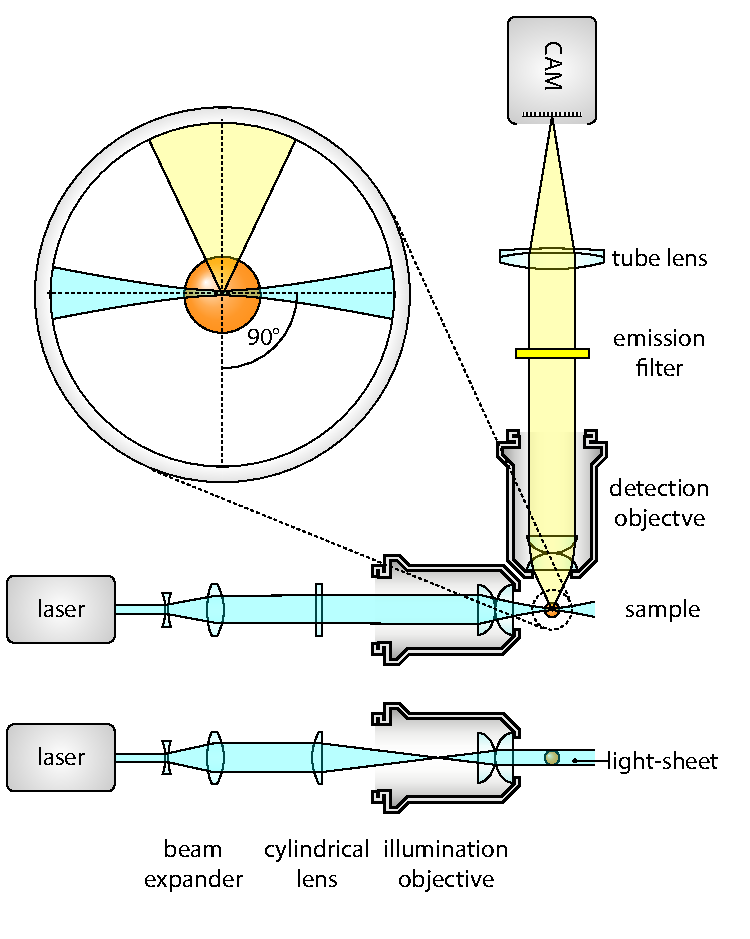
\includegraphics[page=1,width=0.8\textwidth]{spim_cyl}
    \caption{\textbf{Basic optical components of a SPIM.} A selective plane illumination microscope uses two objectives orthogonally aligned. One objective is used to generate a thin light-sheet that illuminates the sample from the side, while the other is used for detection. To generate an image of the specimen, a suitable tube lens is used to focus the light on the sensor of a detection unit (e.g. sCMOS camera). The light-sheet is generated by the illumination objective, using a beam that is previously shaped by a cylindrical lens.}
    \label{fig:light-sheet}
\end{figure}


\subsection{Detection}
The detection unit of a SPIM is basically equivalent to a detection unit of a wide-field microscope, without a dichroic mirror (Figure \ref{fig:light-sheet}). Most important components are the objective together with the tube lens, filter wheel, and a sensor, typically a CCD or sCMOS camera.

One of the most important aspects that determine the resolution of the microscope is the detection objective. Since in developmental biology specimens require a water-based solution, these objectives are usually water dipping objectives directly submerged in the medium. Since the refraction index of water ($n=1.333$) is greater than the refraction index of air, these objectives tend to have a higher $NA$, which results in higher resolution. This, however, also depends on the sensor used, mainly on the pixel size ($d_{sensor}$).

The magnification is typically $10\times$, $20\times$, $40\times$ or $100\times$ but these values are sound only when the objective is used together with the prescribed tube lens. These lenses are specially made to be used with the specific objectives, and are corrected for any aberrations. They typically have a focal length of 160--200mm.

\subsection{Illumination}

\subsubsection{Using cylindrical lens}
The light-sheet can be generated using a cylindrical lens, which focuses the laser beam in only one direction, and creating a thin sheet in the proximity of the focal point. However, to achieve light-sheets that are thin enough, one would need to use cylindrical lens with low focal lengths, but these are hardly accessible in well corrected formats. For this reason, its more common to use a longer focal length cylindrical lens in conjunction with a microscope objective, which is well corrected for chromatic and spherical aberrations \cite{greger_basic_2007}. This way, the light-sheet length, thickness and width can be adjusted for the specific imaging tasks.

For paraxial waves, i.e. waves with nearly parallel wave front normals, a general wave equation can be approximated with the paraxial Helmholz equation \cite{krzic_multiple-view_2009, saleh_fundamentals_2007}
\begin{equation}
    \nabla_T^2 + i 2k \frac{\partial U}{\partial z} = 0
    \label{eq:helmholtz}
\end{equation}
where $\nabla_T^2 = \frac{\partial^2}{\partial x^2} + \frac{\partial^2}{\partial y^2}$, $U(\vec{r})$ is the wave-function, $k=\frac{2\pi}{\lambda}$ is the wavenumber and we assume, that the light spreads in $z$ direction.
 
A simple solution to this differential equation is the Gaussian beam:
\begin{equation}
    U(r,z) = A_0 \cdot \frac{W_0}{W(z)} \cdot e^{-\frac{r^2}{W^2(z)}}\cdot e^{-i\cdot \phi(r,z)}
\label{eq:gaussian}
\end{equation}
where $A_0$ is the amplitude of the wave, $W_0$ is the radius of the beam waist (the thinnest location on the beam), $r=\sqrt{x^2+y^2}$ is the distance from the center of the beam, $W(z)$ is the radius of the beam $z$ distance from the waist, and $\phi(r,z)$ is the combined phase part of the wave-function. Furthermore:

\begin{equation}
    W(z) = W_0\sqrt{1+\left( \frac{z}{z_0} \right)^2}
\end{equation}
where the parameter $z_0$ is called the Rayleigh-range. This has the following connection with the beam waist:

\begin{equation}
    z_0 = \frac{\pi W_0}{\lambda}
\end{equation}
Which means, the thinner the beam waist, the shorter the Rayleigh-range, that is the beam divergence is faster for more focused beams.

Intensity of the emitted fluorescence is based on the intensity of the excitation light. In case of a Gaussian beam:
\begin{equation}
    I(r,z) = U(r,z)\cdot U^*(r,z) = |A_0|^2 \cdot \left( \frac{W_0}{W(z)}\right)^2 \cdot e^{-\frac{2r^2}{W^2(z)}}
\end{equation}

Apart from the circular Gaussian beam, the elliptical Gaussian beam is also an eigenfunction of Helmholtz equation (\ref{eq:helmholtz}):
\begin{equation}
    U(x,y,z) = A_0 \cdot \sqrt{\frac{W_{x,0}}{W_x(z)}} \sqrt{\frac{W_{y,0}}{W_y(z)}} \cdot e^{-\frac{x^2}{W_x^2(z)}} \cdot e^{-\frac{y^2}{W_y^2(z)}} \cdot e^{-i\cdot \phi(x,y,z)}
\end{equation}

This beam still has a Gaussian profile along the $x$ and $y$ axes, but the radii are uncoupled, which results in an elliptical beam. Since the beam waist is different along the two axes, the Rayleigh range is also different:
\begin{align}
    z_{x,0} = \frac{\pi W_{x,0}^2}{\lambda} \\
    z_{y,0} = \frac{\pi W_{y,0}^2}{\lambda}
\end{align}
Intensity of the beam is the following:
\begin{equation}
    I(x,y,z) = U(x,y,z)\cdot U^*(x,y,z) = |A_0|^2 \cdot \frac{W_{x,0}}{W_x(z)} \cdot \frac{W_{y,0}}{W_y(z)} \cdot e^{-\frac{2x^2}{W_x^2(z)}} \cdot e^{-\frac{2y^2}{W_y^2(z)}}
\end{equation}
where
\begin{align}
W_x(z) = W_{x,0}\sqrt{1+\left( \frac{z}{z_{x,0}} \right)^2}\mathrm{\quad and \quad } W_y(z) = W_{y,0}\sqrt{1+\left( \frac{z}{z_{y,0}} \right)^2}
\end{align}

Since the illumination is uneven, the usable field of view is smaller than the actual illuminated region (Figure \ref{fig:fov}). The width of the field of view $w_{fov}$ is determined by the Rayleigh length, since this is in a direct relation with the beam divergence. To stay in the optimal region, the light-sheet should only be used in the range of 1 Rayleigh length on both sides of the beam waist (Figure \ref{fig:width}). In this range, the ratio between the thickest (at $z=z_0$) and the thinnest (at $z=0$) part of the beam $W(z)$ will be $\sqrt{2}\approx 1.4142$ which is still acceptable.

Light-sheet height is determined by the profile of the beam along the vertical axis (Figure \ref{fig:height}). Since this is a Gaussian function (see Equation \ref{eq:gaussian}), only a small part in the middle can be used for imaging, because towards the sides the intensity dramatically drops. To allow a maximum 80\% drop of intensity at the edges, the light-sheet height is $h_{fov}=2\cdot 0.472\cdot W_{x,0}$
\begin{figure}[b!]
    \centering
    \begin{subfigure}[b]{0.7\textwidth}
        \centering
        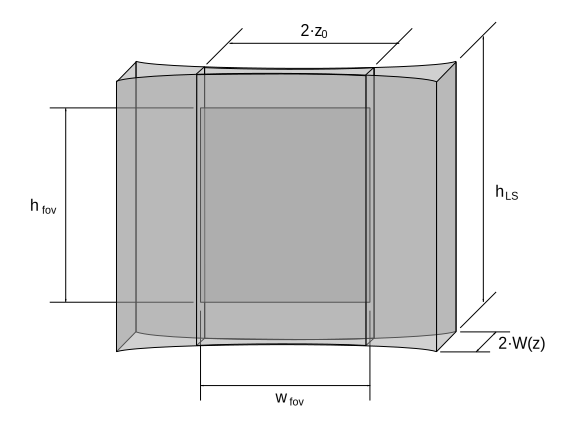
\includegraphics[width=\textwidth]{FOV}
        \caption{}
        \label{fig:fov}
    \end{subfigure}
    \begin{subfigure}[b]{0.49\textwidth}
        \centering
        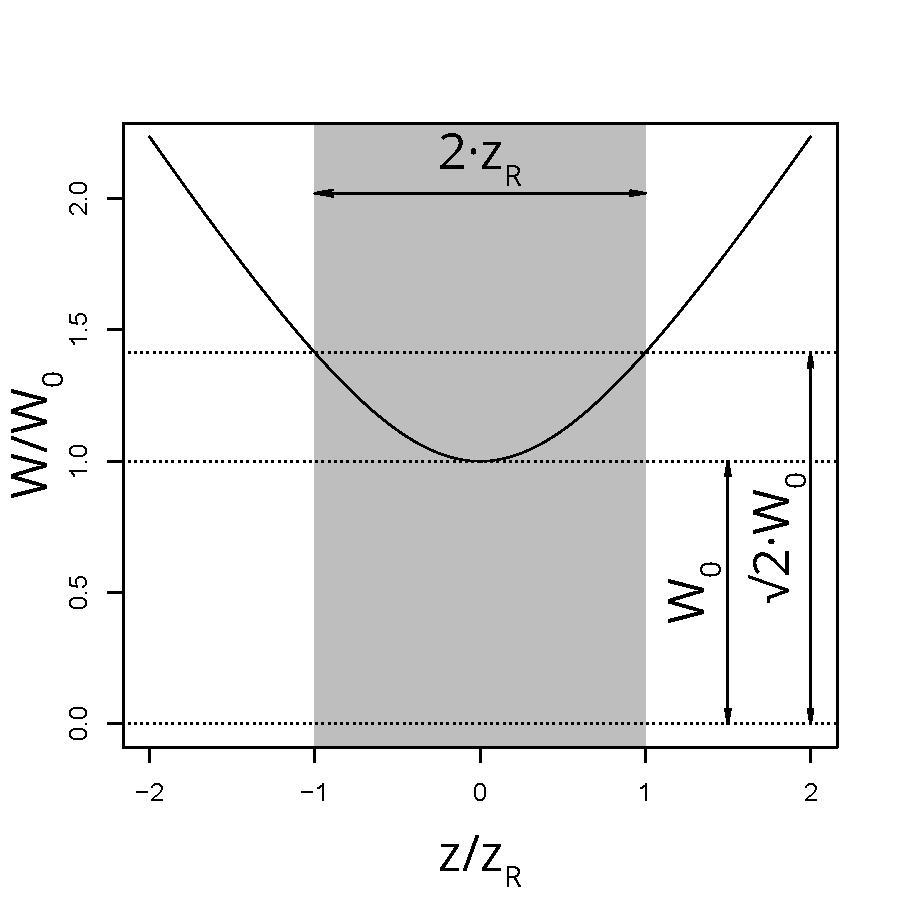
\includegraphics[width=\textwidth]{width}
        \caption{}
        \label{fig:width}
    \end{subfigure}
    \begin{subfigure}[b]{0.49\textwidth}
        \centering
        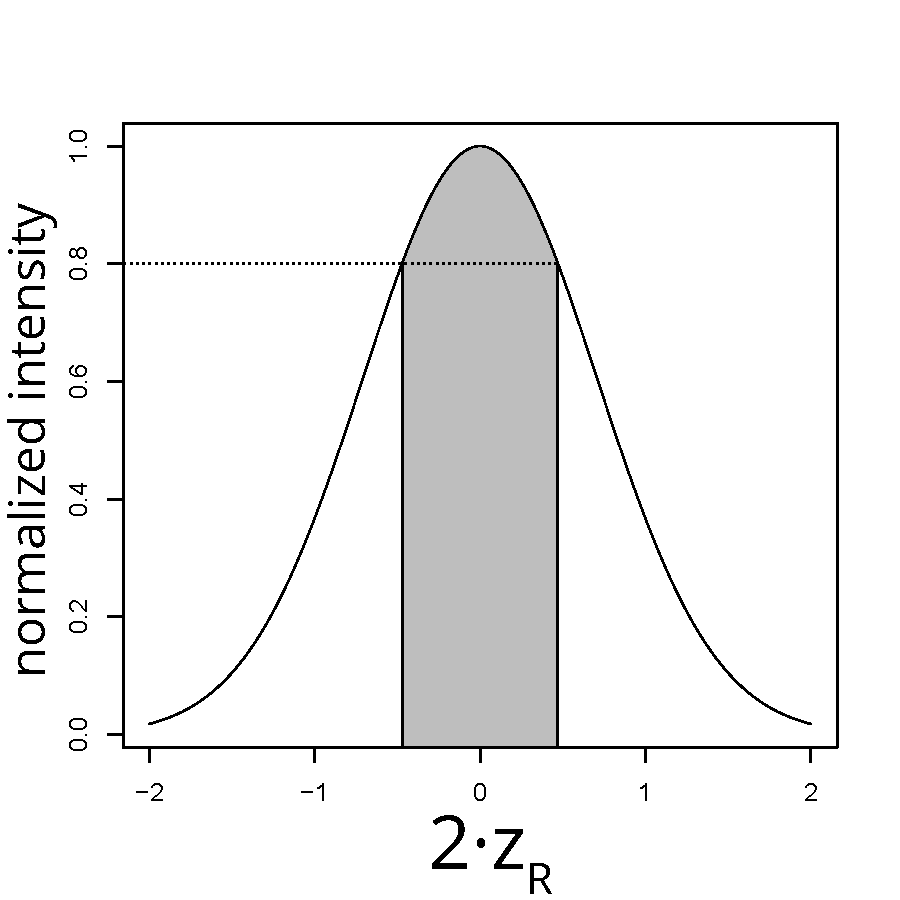
\includegraphics[width=\textwidth]{height}
        \caption{}
        \label{fig:height}
    \end{subfigure}
    \caption{\textbf{Light-sheet dimensions.} \ref{fig:fov} shows a light sheet, with the field of view indicated. Since the light-sheet intensity is uneven, the field of view has to be confined to a smaller region. \ref{fig:width} The width and thickness of the field of view depends on the Rayleigh length of the beam ($z_{y,0}$). \ref{fig:height} Height of the field of view is determined by the Gaussian profile of the elliptical beam.}
    \label{fig:ls_dim}
\end{figure}

\subsubsection{Using focused beam scanning}
\begin{figure}[hbt]
    \centering
    \includegraphics[page=2,width=0.8\textwidth]{spim_cyl}
    \caption{\textbf{DSLM illumination.} DSLM illuminates a specimen by a circularly-symmetric beam that is scanned over the field of view. This creates a virtual light-sheet, which illuminates a section of a specimen just like the SPIM. Light-sheet in DSLM is uniform over the whole field of view and its height can be dynamically altered by changing the beam scan range.
}
    \label{fig:dslm}
\end{figure}

Since using cylindrical lenses it's not possible to generate a homogeneous light-sheet, moreover at higher magnification the Rayleigh range would be too small, we also consider using focused beam scanning to generate the light-sheet (digital scanned light-sheet microscopy, DSLM). To generate a scanning beam, a galvanometer controlled mirror is used to alter the beam path. This can quickly turn around its axis which will result in an angular sweep with the laser beam. To change the angular movement to translation, a scan lens is used to generate an intermediate scanning plane. This plane is then imaged to the specimen by the tube lens and the illumination objective, resulting in a scanned focused beam.

This method to generate the light-sheet has several advantages compared to a static light-sheet. The height of this sheet is not determined by the cylindrical lens, but it can be dynamically modified. Also, the intensity is uniform through the whole height of the light-sheet.

\section{Multi-view light-sheet microscopy}
already in 1989 multi-view to increase axial resolution in conventional optical microscope. They imaged \textit{Drosohpila} metaphase plate in Zeiss Axiomat microscope using a 63x 1.2 NA water immersion objective lens. To increase the axial resolution, a special rotation stage was constructed, that allowed rotation around the object of interest to image it from a 90\si{\degree} tilted view. Using a fusion method in the Fourier space, the resolution increased to \SI{0.25}{\micro\meter} in lateral and \SI{0.4}{\micro\meter} in the axial direction for real samples.

Multiple imaging axis microscopy (MIAM) \cite{swoger_multiple_2003}
to image specimens from 4 directions in a tetrahedral objective configuration, could reach a 5.8 fold increase in axial resolution by combining the four views as a weighted average.
Follow up for this: sample manipulation with optical tweezers / optical levitation in 3D \cite{huisken_three-dimensional_2007}(because of the lack of space for mechanical translation stage)
positioning of a \SI{20}{\micro m} latex bead in a \SI{100}{\micro m} diameter volume by changing the intensity of 4 laser beams. 

\section{SPIM improvements}
things to improve: resolution
axial resolution relative to lateral
complete view
reduce scattering